\documentclass[a4paper,abstract=on]{scrartcl}

\usepackage{todonotes}
\usepackage{../../common/naps62}

\titlehead{%
\tododone{identificação e tema}%
University~of~Minho\hfill Informatics~Department%
}

\subject{Dissertation for Master’s Degree in Informatics Engineering}

\author{%
Miguel~Palhas\\\student\\\email{pg19808@alunos.uminho.pt}%
\and Alberto~Proença\\\advisor\\\email{aproenca@di.uminho.pt}%
\and Luis~Paulo~Santos\\\coadvisor\\\email{psantos@di.uminho.pt}%
}

\title{An Evaluation of the GAMA Framework for Heterogeneous Platforms: The Progressive Photon Mapping Algorithm}

\date{Braga, February 2013}

\begin{document}

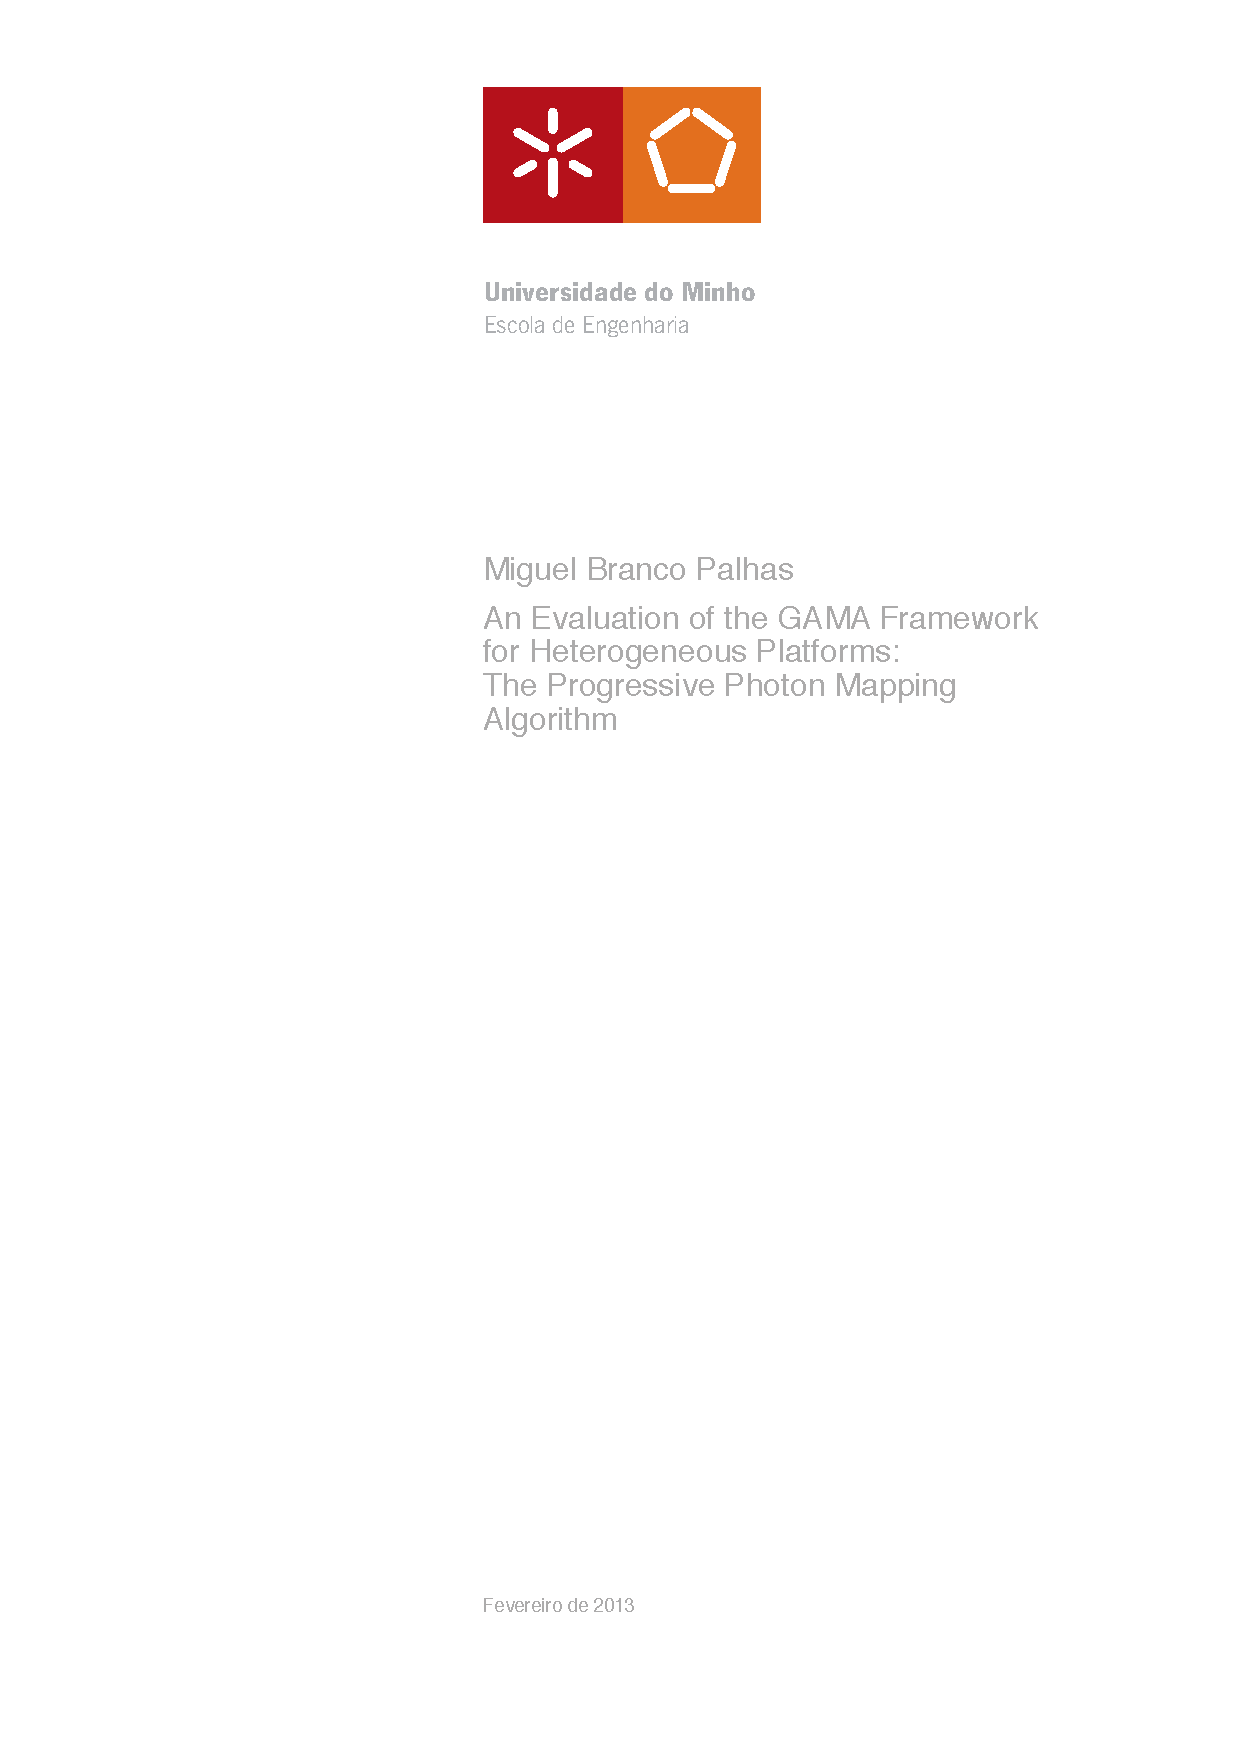
\includepdf[pages=-]{misc/cover-mei}
\maketitle

%
% include all tex/ files
%
\bash[stdoutFile=/dev/null,stderrFile=/dev/null,exitCodeFile=/dev/null,scriptFile=bash.out]
ls tex/ | egrep ^[^_A-Z] | sed "s/\([0-9][^.]*\)\.tex/\\\\subfile{tex\/\1}/" > tex/_sections.tex
\END

\input{tex/_sections}

\appendix
\bash[stdoutFile=/dev/null,stderrFile=/dev/null,exitCodeFile=/dev/null,scriptFile=bash.out]
ls tex/ | egrep ^[^_0-9] | sed "s/\([A-Z][^.]*\)\.tex/\\\\subfile{tex\/\1}/" > tex/_appendixes.tex
\END
\input{tex/_appendixes}


\end{document}
